\PassOptionsToPackage{subsection=false}{beamerouterthememiniframes}
\documentclass[8pt]{beamer}

\usepackage[utf8]{inputenc}
\usepackage[T1]{fontenc}
\usepackage{lmodern}
\usepackage{amsmath}
\usepackage[normalem]{ulem}
\usepackage{tikz}
\usepackage{hyperref}
\usepackage{listings}
\usepackage{color}
\usepackage{fancyvrb}
\usepackage{minted}

\usepackage{mathptmx}
\usepackage[scaled=0.9]{helvet}

\definecolor{links}{HTML}{2A1B81}
\hypersetup{colorlinks,linkcolor=,urlcolor=links}

\usetikzlibrary{shapes,arrows,automata}

\tikzset{
  vertex/.style={
    rectangle,
    rounded corners,
    draw=black, thick,
    text centered
  },
}

\mode<beamer>
{
  \usetheme{Frankfurt}
  \useoutertheme{miniframes}
  \setbeamercovered{transparent}
}

\subject{Talks}

\AtBeginSection[]
{
  \begin{frame}<beamer>{}
    \tableofcontents[currentsection]
  \end{frame}
}

\title[LLVM]{LLVM: Low Level Virtual Machine\\Theory and practice}
\author[Krystian Bacławski]{\href{mailto:cahirwpz@cs.uni.wroc.pl}{Krystian Bacławski}}
\institute{Computer Science Department\\University of Wrocław}
\date{\today}

\begin{document}

\begin{frame}
\titlepage
\end{frame}

\section[Theory]{Theoretical overview}
\subsection*{Theory}

\begin{frame}{Stream of instructions}
  \begin{block}{What really does CPU execute?}
    \begin{itemize}
      \item Data flow instructions.
      \item Control flow instructions.
      \item Implicitly organized into Control Flow Graph (CFG).
    \end{itemize}
  \end{block}

  \begin{block}{What is Control Flow Graph?}
    \begin{itemize}
      \item A directed graph.
      \item Each node stores a sequence of data flow instructions \ldots
      \item and finishes with exactly one control flow instruction.
      \item Entry point to each node is labelled.
      \item Control flow instruction include: direct jump, indirect jump,
        function call / return, conditional branch, exception.
      \item Edges are determined by behaviour of the last instruction.
      \item $\forall n \in V. pred(n) \ge 1 \lor succ(n) \ge 1$
    \end{itemize}
  \end{block}
\end{frame}

\begin{frame}{Control Flow Graph terminology}
  \begin{block}{Blocks}
    \begin{description}
      \item[BB] Basic block is a node of CFG.
      \item[Entry block] Has no predecessor (source).
      \item[Exit block] Has no successors (sink).
      \item[EBB] Linear sequence of basic blocks, which can be entered from outside only through one node.
    \end{description}
  \end{block}

  \begin{block}{Edge}
    \begin{description}
      \item[back] goes to predecessor (loop)
      \item[critical] $(a,b) \in E$ is critical if $succ(a) > 1 \land pred(a) > 1$ -- requires splitting. 
      \item[abnormal] "dangling" edge -- jump to address not known at compile-time.
    \end{description}
  \end{block}

  \begin{block}{Dominance relation}
    Consider a control flow graph $G$ with two nodes $v$, $w$, and an entry
    block $s$. \\
    If every path from $s$ to $w$ contains $v$, then $v$ dominates $w$, written
    $v \gg w$.
  \end{block}
\end{frame}

\begin{frame}[fragile=singleslide]{Control Flow Graph examples}
  \begin{columns}[c]
    \column{.33\textwidth}
    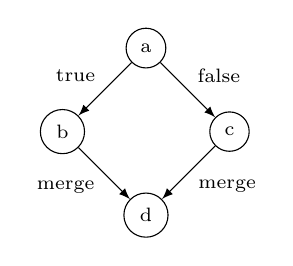
\begin{tikzpicture}[->, font=\scriptsize, >=latex, auto, node distance=1.5cm]
      \tikzstyle{every state}=[circle, draw, minimum size=0.5cm]
      \node[state] (a) {a};
      \node[state] (b) [below left of=a] {b};
      \node[state] (c) [below right of=a] {c};
      \node[state] (d) [below right of=b] {d};
      \path
      (a) edge node[left,yshift=0.5em]{true} (b) 
      (a) edge node[right,yshift=0.5em]{false} (c) 
      (b) edge node[left,yshift=-0.5em]{merge} (d) 
      (c) edge node[right,yshift=-0.5em]{merge} (d);
    \end{tikzpicture}
    \begin{minted}[gobble=6]{c}
      if (a)
        b;
      else
        c;
      d;
    \end{minted}

    \column{.33\textwidth}
    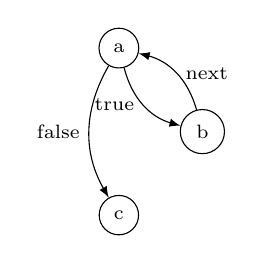
\begin{tikzpicture}[->, font=\scriptsize, >=latex, auto, node distance=1.5cm]
      \tikzstyle{every state}=[circle, draw, minimum size=0.5cm]
      \node[state] (a) {a};
      \node[state] (b) [below right of=a] {b};
      \node[state] (c) [below left of=b] {c};
      \path 
      (a) edge [bend right=30] node[left]{true} (b)
      (b) edge [bend right=30] node[right]{next} (a)
      (a) edge [bend right=30] node[left]{false} (c);
    \end{tikzpicture}
    \begin{minted}[gobble=6]{c}
      while (a)
        b;
      c;
    \end{minted}

    \column{.33\textwidth}
    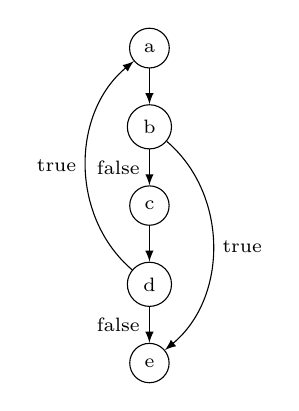
\begin{tikzpicture}[->, font=\scriptsize, >=latex, auto, node distance=1.0cm]
      \tikzstyle{every state}=[circle, draw, minimum size=0.5cm]
      \node[state] (a) {a};
      \node[state] (b) [below of=a] {b};
      \node[state] (c) [below of=b] {c};
      \node[state] (d) [below of=c] {d};
      \node[state] (e) [below of=d] {e};
      \path
      (a) edge (b)
      (b) edge [bend left=50] node[right]{true} (e)
      (b) edge node[left]{false} (c)
      (c) edge (d)
      (d) edge [bend left=50] node[left]{true} (a)
      (d) edge node[left]{false} (e);
    \end{tikzpicture}
    \begin{minted}[gobble=6]{c}
      do
      {
        a;
        if (b)
          break;
        c;
      } while (d);
      e;
    \end{minted}
  \end{columns}
\end{frame}

\begin{frame}[fragile]{SSA form}
  \begin{figure}
    \centering
    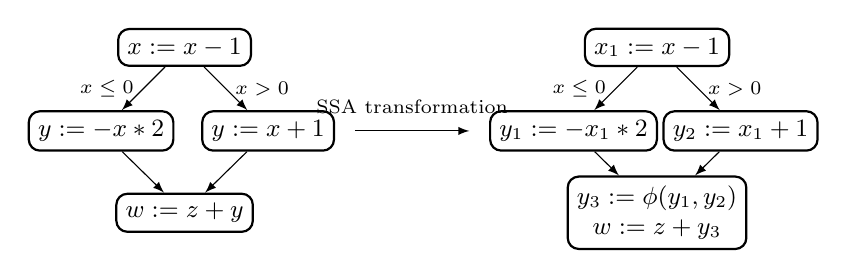
\begin{tikzpicture}[auto,node distance=1.5cm,font=\small]
      \begin{scope}
        \node[vertex] (a) {$x := x - 1$};
        \node[vertex, below left of=a] (b) {$y := -x * 2$};
        \node[vertex, below right of=a] (c) {$y := x + 1$};
        \node[vertex, below of=a,yshift=-0.6cm] (d) {$w := z + y$};
        \path[->,font=\scriptsize,>=latex]
        (a) edge node[left]{$x \leq 0$} (b)
        (a) edge node[right]{$x > 0$} (c)
        (b) edge (d)
        (c) edge (d);
      \end{scope}

      \begin{scope}[xshift=6cm]
        \node[vertex] (a') {$x_1 := x - 1$};
        \node[vertex, below left of=a'] (b') {$y_1 := -x_1 * 2$};
        \node[vertex, below right of=a'] (c') {$y_2 := x_1 + 1$};
        \node[vertex, below of=a',yshift=-0.6cm,align=center]
        (d') {$y_3 := \phi(y_1,y_2)$ \\ $w := z + y_3$};
        \path[->,font=\scriptsize,>=latex]
        (a') edge node[left]{$x \leq 0$} (b')
        (a') edge node[right]{$x > 0$} (c')
        (b') edge (d')
        (c') edge (d');
      \end{scope}

      \draw [->,>=latex,shorten >=2.5mm,shorten <=2.5mm] (c) -- (b')
      node [above=1mm,font=\scriptsize,midway,text centered] {SSA transformation};
    \end{tikzpicture}
    \caption{Example of SSA transformation for simple \texttt{if-then-else} statement.}
  \end{figure}

  \begin{block}{\textit{Static Single Assignment} form properties}
    \begin{itemize}
      \item Variables propagate along edges.
      \item Variables, once assigned, cannot be changed!
      \item $\phi(\ldots)$ operator merges value which flows down from several nodes.
      \item Thanks to immutability better properties for code analysis
        algorithms.
      \item Some optimizations are available almost for free (eg. dead code
        elimination).
    \end{itemize}
  \end{block}
\end{frame}

\begin{frame}{Compilation process}
  % There's well known algorithm to transform code into SSA form (dominance frontiers).

  \begin{block}{Code analysis and transformations}
    \begin{itemize}
      \item High-level -- language specific.
      \item Intermediate level -- generic optimizations for different languages
        (predominantly some form of CFG with SSA instructions).
      \item Code generation -- processor specific.
    \end{itemize}
    \textbf{Depending on the language low-level details are important at each
      level -- think of GPGPUs or other specialised architectures.}
  \end{block}

  \begin{block}{Lowering}
    When we're done with optimizations and analysis at given level we have to
    perform lowering phase. It has to correctly transform one code form to
    another.
  \end{block}

  \begin{alertblock}{Implications?}
    \begin{itemize}
      \item Each time lowering looses information! (about types, program
        structure, etc.)
      \item How to make association between program counter and source line?
    \end{itemize}
  \end{alertblock}
\end{frame}

\begin{frame}{Optimisations}
  \begin{block}{Compilation unit (module or object)}
    Defines several symbols that refer to functions, global variables and other
    resources specific to the language. Symbols are usually untyped, have
    assigned visiblity and other linkage attributes.
  \end{block}

  \begin{block}{Scope}
    We can optimize or analyse the code at several levels:
    \begin{itemize}
      \item instruction window -- instruction scheduling and selection,
      \item function -- constant folding, loop optimizations,
      \item inter-procedural optimizations (IPO) -- e.g. inlining and specialisation.
      \item link-time optimizations (LTO) -- aka inter-module optimizations.
    \end{itemize}
  \end{block}
\end{frame}

\section[Practice]{Practical considerations}
\subsection*{Practical considerations}

\begin{frame}{Processor model}
  \begin{block}{RISC architecture}
    \begin{itemize}
      \item Most instructions have three operands.
      \item Load-store architecture.
      \item Register machine (floating-point, integer).
      \item Finite number of architectural registers (usually 32).
      \item Minimal hardware support for stack.
      \item Few machine types (integers of different width).
      \item Instructions carry information how to interpret data in registers or memory.
      \item Simple conditional jumps (NE, EQ).
    \end{itemize}
  \end{block}

  \begin{block}{ISA vs. microarchitecture}
    \begin{itemize}
      \item \textit{Instruction Set Architecture} is an interface between a compiler and the machine.
      \item Processor is a realization of some microarchitecture.
      \item ISA abstracts how CPU actually executes instructions.
      \item There are many ways to execute same instruction stream correctly!
      \item To generate efficient code you have to understand microarchitecture!
    \end{itemize}
  \end{block}
\end{frame}

\begin{frame}{Memory hierarchy}
  \begin{alertblock}{Problems with DRAM}
    Memories are several hundred times slower than registers. Memory technology
    could not follow up processors for last 30 years! Processors can calculate
    very quickly, but how to feed them with instruction and data at a desired
    rate.
  \end{alertblock}

  \begin{block}{Locality}
    Human-written code exposes memory access locality:
    \begin{description}
      \item[temporal] reference same data over and over (variables),
      \item[spatial] reference nearby location (data structures).
    \end{description}
    \vspace{1em}
    How to exploit locality?
    \begin{itemize}
      \item Cache memory -- stores working set, block transfer.
      \item Delayed writing -- write-back policy.
      \item Prefetching and speculative loads.
    \end{itemize}
    \vspace{1em}
    \textbf{Compilers perform cache-aware optimizations but only w.r.t.
      instruction stream.}
  \end{block}
\end{frame}

\begin{frame}{Memory model}
  \begin{alertblock}{}
    Instruction results and side-effect may become observable with some delay,
    especially in multiprocessor NUCA systems.
  \end{alertblock}

  \begin{block}{Consistency model}
    \begin{description}
      \item[strict] a read operation shall return the value written by the
        most recent store operation,
      \item[sequential] the result of an execution is the same as a single
        interleaving of sequential, program-order access from different
        processors,
      \item[processor] writes from a process are observed by other clients to
        be in program order; all clients observe a single interleaving of
        writes from different processors,
      \item[partial store order] freely reorder local writes with respect to
        other local writes,
      \item[weak] freely reorder local writes ahead of local reads,
      \item[release] when software does \textit{acquire} or \textit{release},
        the memory system updates all protected variables before continuing
        (memory barrier instruction needed).
    \end{description}
    \textbf{Compilers have to know the model -- otherwise they cannot apply
      certain optimisations!}
  \end{block}
\end{frame}

\begin{frame}[fragile]{ILP}
  \begin{block}{Instruction Level Parallelism}
    Modern processors are able to "execute" multiple instructions at once -- an
    order of 100 is not uncommon. They can issue several instruction from BB at
    once and can speculate execution of successive BBs.
  \end{block}

  \begin{block}{Hazards}
    Control and data hazards limit ILP and thus processors throughput.
    \begin{description}
      \item[control] conditional branches, indirect jumps, exceptions
      \item[RAW] real dependency (limits data flow)
        \begin{Verbatim}[commandchars=\\\{\}]
          \underline{R2} <- R1 + R3
          R4 <- \underline{R2} + R3
        \end{Verbatim}
      \item[WAR] anti-dependency
        \begin{Verbatim}[commandchars=\\\{\}]
          R4 <- R1 + \underline{R5}
          \underline{R5} <- R1 + R2
        \end{Verbatim}
      \item[WAW] output dependency
        \begin{Verbatim}[commandchars=\\\{\}]
          \underline{R2} <- R4 + R7
          \underline{R2} <- R1 + R3
        \end{Verbatim}
    \end{description}
  \end{block}
\end{frame}

\begin{frame}{ILP exploitation techniques}
  \begin{alertblock}{}
    Many papers about observed ILP. Conclusions not decisive -- advancements in
    compiler and processor technology change assumptions every couple of years.
  \end{alertblock}

  \begin{block}{Most successful techniques}
    \begin{itemize}
      \item Divide instruction execution into phases -- pipelining.
      \item Analyse data hazards and try to issue several instructions per
        clock cycle.
      \item Allow to execute instructions out of order.
      \item Avoid \textbf{WAR} and \textbf{WAW} with register renaming.
      \item Employ aggressive branch prediction to speculate instruction execution.
    \end{itemize}
  \end{block}

  \begin{alertblock}{}
    Processors effectively perform dynamic analysis on the running code. Having
    extra internal registers they partially undo suboptimal register assignment.
    Fragments of CFG is partially recovered thanks to trace caches.\\
    \vspace{1.0em}
    \textbf{Widely accepted methods of program encoding seems to be highly
      ineffective!}
  \end{alertblock}
\end{frame}

\begin{frame}{Microarchitecture}
  \begin{figure}
    \centering
    \includegraphics[width=0.75\textwidth]{microarchitecture.png}
    \caption{Common framework for modern microarchitectures.}
  \end{figure}
\end{frame}

\begin{frame}{Application Binary Interface}
  \begin{block}{Symbols and name mangling}
    \begin{itemize}
      \item A mapping from identifier and object's type into a link-time symbol.
      \item Do we need to encode function's signature into a symbol (due to overloading)?
      \item Any attributes associated with a symbol (visibility, linking, optimization)?
    \end{itemize}
  \end{block}
    
  \begin{block}{Function calling convention}
    \begin{itemize}
      \item Where to put arguments (stack or registers)?
      \item Where the result is available?
      \item How to create activation record?
      \item Which registers need to be saved and restored?
    \end{itemize}
  \end{block}

  \begin{block}{Data and memory organization}
    \begin{itemize}
      \item Which bit is MSB and LSB?
      \item Big-endian or little-endian?
      \item Alignment requirements for words?
      \item Size of machine data types (integer, float, etc.)?
    \end{itemize}
  \end{block}
\end{frame}

\begin{frame}{Linking \& running}
  \begin{block}{Static and dynamic linkers}
    \begin{itemize}
      \item Handle loadable and linkable files specific for particular OS.
        ELF is specified by ABI.
      \item Handle cross-references at link-time -- modules contain a
        list of symbols and relocations.
      \item Code intended for dynamic linking must be compiled separately.
      \item Dynamic linker lives as a part of program (lazy binding, on-demand
        loading).
    \end{itemize}
  \end{block}

  \begin{block}{Run-time environment}
    Is specific to every language, however they share common functionalities:
    \begin{itemize}
      \item start-up code -- quite complex entity that calls "main" function,
      \item set of basic functions as defined by language specification,
      \item dynamic loader / linker -- to import binary modules / libraries.
    \end{itemize}
    In higher level languages run-time environment additionally may comprise of:
    \begin{itemize}
      \item coroutines library -- lightweight threads, continuations,
      \item stack unwinding -- exceptions and other non-local jumps,
      \item foreign function interface -- for calling C language libraries,
      \item garbage collector -- either accurate or conservative,
      \item \ldots and other low-level routines not expressible in the language.
    \end{itemize}
  \end{block}
\end{frame}

\begin{frame}{}
  \vspace*{\stretch{2}}
  \begin{center}
    {\Huge Questions?}
  \end{center}
  \vspace{\stretch{3}}
\end{frame}

\end{document}
